\nxsection{Le r\^ole ''Caissier''}\label{sec:utilisateurs-lecaissier}
\index{caissier}
\index{LeCaissier}

La figure~\ref{fig:fenetre-principale-caissier} illustre la
fen\^etre d'acceuil d'un utilisateur avec le \role \caissier,
apr\`es qu'il se soit enregistr\'e dans \yeren.\\

\begin{figure}[!htbp]
\centering
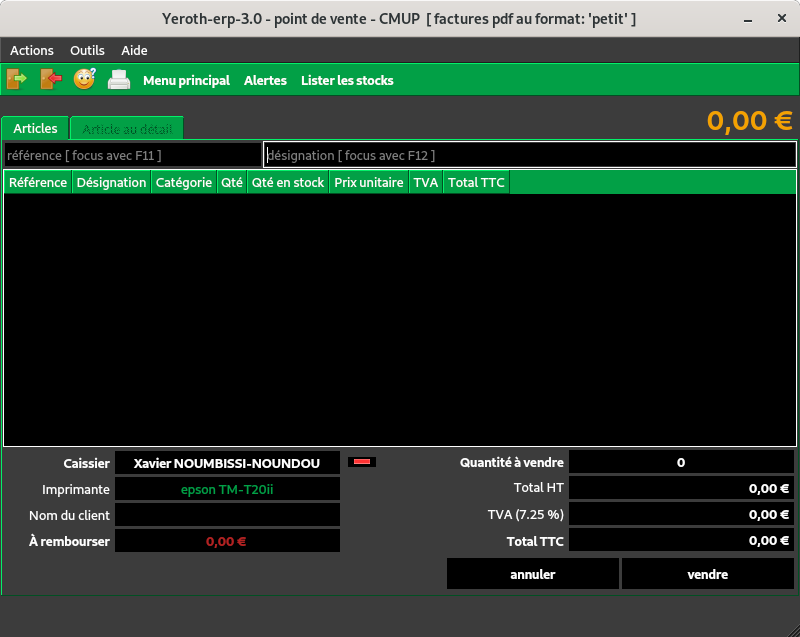
\includegraphics[scale=0.63]{images/yeren-fenetre-caissier.png}
\caption{La fen\^etre d'acceuil d'un caissier.}
\label{fig:fenetre-principale-caissier}
\end{figure}

Un utilisateur de \yeren avec le \role "\caissier" assume
les t\^aches suivantes:
\begin{enumerate}[1)]
	\item lister les stocks \`a partir de l'interface de vente	
	\item visualiser une facture proforma		
	\item imprimer une facture proforma
	\item vendre un ou plusieurs stocks (ou articles).\\
\end{enumerate}